\documentclass[a4paper,10pt]{article}
\usepackage[utf8x]{inputenc}
\usepackage{graphicx}
\usepackage{gb4e}
\usepackage{qtree}
\usepackage{amssymbib}
%opening
\title{Modeling the relation between proto-languages and language families}
\author{Sebastian Nordhoff}

\begin{document}

\maketitle

\begin{abstract}

\end{abstract}

\section{Introduction}

language classifications
    Ethnologue
    Multitree Composite
\ea
Indo-European \\
.\hspace{.2cm}Middle Indo-European \\
.\hspace{.4cm}Late Indo-European \\
.\hspace{.6cm}Germanic \\
.\hspace{.8cm}Northwest Germanic\\
.\hspace{1cm}West Germanic \\
.\hspace{1.2cm}North Sea Germanic \\
.\hspace{1.4cm}Old English [ang]\\
.\hspace{1.6cm}Anglian \\
.\hspace{1.8cm}Mercian \\
.\hspace{2cm}Middle English [enm]\\
.\hspace{2.2cm}English [eng]
\z

When interpreting the above tree, we can make a number of observations. We can say for instance that two adjacent nodes are in a childOf-relation. For instance, \em Middle Indo-European \em is a child of \em Indo-European\em, \em Germanic \em is a child of \em Late Indo-European\em, \em West Germanic \em is a child of \em Northwest Germanic\em, \em Old English \em is a child of \em North Sea Germanic\em, and so on.

A closer inspection, however, reveals that the nodes of this tree actually fall into two different sets. Some of them denote sets of languages, like \em West Germanic\em, others denote historic varieties, like \em Old English\em. 


We can identify the sets by evaluating the proposition `X is a subset of Y ' for adjacent nodes.

\ea
\ea \em West Germanic \em is a subset of \em Northwest Germanic\em 
\ex *\em Old English \em is  a subset of \em West Germanic\em 
\ex *\em Anglian \em is a subset of \em Old English\em.\z
\z

Historic varieties can be identified by evaluating the proposition `X is a later variety of Y':

\ea
\ea \em English \em is a later variety of \em Middle English\em  
\ex *\em Middle English \em is  a later variety of  \em Mercian\em.  
\ex *\em Anglian \em is a later variety of \em Old English\em.\z
\z

These are two important insights about the relation between languages and language families of Northwestern Europe at different points in time, but they should be kept distinct conceptually and the difference should be made explicit. At the same time, one would not want to completely dissociate the two, as there are obvious interconnections which can inform the historical linguist. How this conceptual separation can be achieved while maintaining the insights contained in the `traditional' tree will be the topic of the remainder of this paper. I will show this on a stammbaum model as customary, which still seems to be the most popular model of representing language history. Future research will deal with the modeling of areality.



Both of the predicates just discussed are transitive:

\ea \em English \em is a later variety of \em Old English \em\z
\ea \em Anglian \em is a subset of \em Indo-European \em\z

Section \ref{} will show
 
Section \ref{} will show
 
Section \ref{} will show
 
\section{How to define languages and language families: a resource based approach}
The model proposed here is inscribed into a resource-based framework. Languages in the context of linguistic investigation are seen as a the collection of verifiable things we know about them. `English' is the collection of everything ever written on English, `Tocharian' is the collection of everything every written on Tocharian and so on. Note that there are some communication systems used by humans which will not be considered under this approach: those are the ones of which we have no documentation. This shortcoming is acceptable as these languages could not be classified anyway. While such languages certainly still exist on Earth,  they have no bearing on issues of language classification while they are unknown. The second part of the definition is `verifiable'. This excludes personal knowledge, personal communication, hearsay, conjectures etc. It must be possible for a dedicated researcher to trace the resources which form part of the definitional set used for a language. Note that the normal case for a resource is to be written, but audio or video resources are equally legitimate.

Within the set of 8031 languages in our database which have an official ISO 639-3 code, we have identified 6307, or 79\%, which have at least one resource which treats them. We are still working on establishing the definitional set for the remainder. The amount of documentation available for the different languages is plotted in Figure \ref{fig:amountofdocumentation}

\begin{figure}
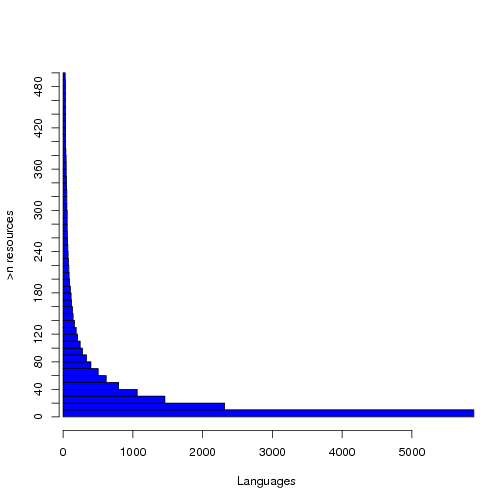
\includegraphics[height=.3\textheight]{docstats.png}
\caption{Number of languages which exceed a given number of resources. About 6000 languages have at least one resource; about 2200 of those have more than 10; about 1300 of those have more than 20 and so on. Only about 200 languages have more than 100 resources.}
\label{fig:amountofdocumentation}
\end{figure}


        no fiat languages

        Good, Nordhoff \& Hammarström ISWC

            problems with fiat languages

\section{Definitions}
We will handle the following concepts when modeling the relation between languages: \em lectodocs\em, \em doculects\em, and \em languoids\em. These will now be defined in turn.

\subsection{Lectodoc}
A lectodoc is a document which contains linguistically relevant information. The crucial point here is that we are dealing with documents, i.e. entities which could be printed. Lectodocs cannot be spoken. Dictionaries and grammatical descriptions are the prototypical lectodocs, but other kinds of work also fall under this definition. Word lists, theoretical articles on a particularly interesting phenomenon found in a language, or phonological descriptions are all documents which provide linguistic information and are therefore lectodocs. The types of documents just listed provide information about the phonological, morphosyntactic or lexical structure of a language. Next to these documents providing structural information, there are also lectodocs which provide information about sociodemographic details. These are equally important. Studies of language use, language variation, language and identity and other sociolinguistics topics come to mind. Related to this are ethnographic studies and census data. A final type of lectodoc are overview works like handbooks, bibliographies and the like. 

\subsection{Doculect}
Cysouw. 

A doculect is a documented linguistic variety (cf. dialect, idiolect, sociolect etc). It is the mental counterpart of a lectodoc. While a lectodoc can be printed, but not spoken, a doculect can be spoken, but not printed.

A doculect is tied to the lectodoc it is described in. This means that we have at least as many doculects as we have lectodocs. This definition entails that the OED and Webster's described different doculects. Actually, the granularity is even greater than that because different editions of the OED also describe different doculects.\footnote{To put it differently, doculects correspond to FRBR `manifestations'.} To capture the intuition that these doculects are not so different after all, we can group them into languoids.

\subsection{Languoid}
A languoid is a collection of doculects. We can group the OED, Websters, and Quirk's grammar of English together and declare that these three doculects all provide information about a languoid we want to call `English'. We have just formed a `terminal' languoid, i.e. a languoid whose members are all doculects. It is also possible to have non-terminal languoids. Nonterminal languoids can contain other languoids. For instance, we could group a number of doculects into a languoid `Dutch' and then group those two languoids together into a larger languoid `West Germanic'. Nonterminal languoids may also contain doculects, e.g. `The Germanic languages'. 

Every languoid is reducible to the doculects contained in it. We call this list its \em Bibliographical Grounding\em.

\section{Illustration}
We will illustrate the three concepts just introduced with an example from Dravidian. We will start with the documents given in Table \ref{tab:dravidiandocs}.

\begin{table}
\begin{tabular}{p{5cm}p{2cm}p{2cm}p{4cm}}
Lectodoc & Doculect & Terminal languoid & Non-terminal languoids\\ 
\hline
Andronov, Michail S.  (1960) Tamil'skij jazyk & Tamil of Andrononov (1960)& Tamil & Tamil-Malayalam, ...,  Southern Dravidian, ..., Dravidian\\
Annamalai, E.  (2000) Lexical anaphors and pronouns in Tamil & Tamil of Annamalai (2000)& Tamil& Tamil-Malayalam, ...,  Southern Dravidian, ..., Dravidian\\
Asher, R. E.  (1985) Tamil & Tamil of Asher (1985)& Tamil& Tamil-Malayalam, ...,  Southern Dravidian, ..., Dravidian\\
Beythan, Hermann  (1943) Praktische Grammatik und Übungsbuch der Tamilsprache & Tamil of Beythan (1943)& Tamil& Tamil-Malayalam, ...,  Southern Dravidian, ..., Dravidian\\
\hline
Andronov, Michail S.  (1993)  Jazyk malajalam  & Malayalam of Andronov (1993) & Malayalam& Tamil-Malayalam, ...,  Southern Dravidian, ..., Dravidian\\
Asher, R.E.  (1968) Existential, possessive, locative and copulative sentences in Malayalam & Malayalam of Asher (1968)& Malayalam & Tamil-Malayalam, ...,  Southern Dravidian, ..., Dravidian\\
Asher, R.E. and T.C. Kumari  (1997) Malayalam & Malayalam of Asher \& Kumari (1997) & Malayalam& Tamil-Malayalam, ...,  Southern Dravidian, ..., Dravidian\\
\end{tabular}
\caption{Lectodocs, doculects, and terminal languoids of some literature on Southern Dravidian.}
\label{tab:dravidiandocs}
\end{table}

These seven lectodocs establish seven different doculects, which are grouped into two terminal languoids, Tamil and Malayalam in this case. The terminal languoids can then be grouped in turn into higher-order non-terminal languoids. The bibliographical grounding of the two terminal languoids and one higher-order languoid is given below:

\begin{itemize}
 \item Tamil: Andronov 1960, Annamalai 2000, Asher 1985, Beythan 1943
 \item Malayalam: Andronov 1993, Asher 1968, Asher \& Kumari 1997
 \item Tamil-Malayalam:Andronov 1960, Annamalai 2000, Asher 1985, Beythan 1943, Andronov 1993, Asher 1968, Asher \& Kumari 1997
\end{itemize}

It is easy to see how this model would continue for higher order languoids like Southern Dravidian or Dravidian.

\subsection{Basic modeling}

concepts

The following relations hold between lectodocs, doculects, terminal languoids and non-terminal languoids:
\begin{itemize}
 \item a lectodoc describes a doculect
 \item a doculect is an element of a languoid
 \item a (terminal or nonterminal) languoid can be the subset of a nonterminal languoid
 \item a lectodoc forms part of the Bibliographical Grounding of a languoid
\end{itemize}

\subsubsection{Terminal languoids}
Terminal languoids have been modeled above and need no further discussion here.

\subsubsection{Non-terminal languoids}
Non-terminal languoids are distinguished from terminal languoids by their including other languoids. Doculects can be included, but this is optional. The following table lists lectodocs whose doculects would be directly included into the languoid `Dravidian' rather than in any of its sublanguoids.

\begin{table}
\begin{tabular}{p{5cm}p{2cm}p{2cm}p{4cm}}
Lectodoc & Doculect & Terminal languoid & Non-terminal languoids\\ 
\hline
Bloch, Jules  (1954) The grammatical structure of Dravidian languages & Dravidian of Bloch 1954 & - & Dravidian\\\\
Burrow, Thomas and Emeneau, M. B.  (1998) A Dravidian etymological dictionary & Dravidian of Burrow \& Emeneau & -& Dravidian\\\\
Caldwell, Robert  (1998) A comparative grammar of the Dravidian or South Indian family of languages & Dravidian of Caldwell 1998 & -& Dravidian\\\\
K. V. Zvelebil  (1990) Dravidian Linguistics: An Introduction & Dravidian of Zvelebil 1990 & - & Dravidian \\\\
Rangaswamy, R.  (1995) Comparative Dravidian & Dravidian of Rangaswamy 1995 & - & Dravidian\\
 \end{tabular}
\caption{Some works which directly attach to the non-terminal languoid `Dravidian'}
\label{tab:nonterminallanguoid}
\end{table}

discussion

\subsubsection{Historical varieties}
We have now seen how the set-theoretic approach can model synchronic family relations between linguistic varieties and associated documents. When we include historical varieties, things become a bit more complicated. We can for instance not equate Tamil-Malayalam with Old Tamil. While it is perfectly legitimate to say that Asher \& Kumari 1997 provide information about Tamil-Malayalam, it is wrong to say that they provide information about Old Tamil. Rather, we have to create a new terminal languoid `Old Tamil', and model its relations to the extant `Tamil', `Malayalam', and `Tamil-Malayalam'. This new languoid has to have Bibliographical Grounding as well. Table \ref{tab:illustrationOldTamil} provides some lectodocs for historic varieties.

\begin{table}
\begin{tabular}{p{5cm}p{2cm}p{2cm}p{4cm}}
Lectodoc & Doculect & Terminal languoid & Non-terminal languoids\\ 
\hline
Lehmann, Thomas  (1991) Grammatik des Alttamil: unter besonderer Berücksichtigung der Cankam-Texte des Dichters Kapilar & Old Tamil of Lehmann 1991 & Old Tamil & Southern Dravidian, Dravidian \\\\
Steever, Sanford B.  (2008) Old Tamil & Old Tamil of Steever 2008 & Old Tamil & Southern Dravidian, Dravidian \\\\
Zvelebil, Kamil and Andronov, Michail S. and Navrozov, L.  (1967) Vvedenie v istoriceskuju grammatiky tamilskogo jazyka & Old Tamil of Zvelebil, Andronov, \& Navrozov 1967 & Old Tamil & Southern Dravidian, Dravidian \\\\
\end{tabular}
\caption{Some works which refer to the historical languoid `Old Tamil'}
\label{tab:nonterminallanguoid}
\end{table}

On an non-formal level, we can formulate the following propositions:

\begin{itemize}
 \item Tamil-Malayalam is the result of breakup of Old Tamil
 \item Tamil-Malayalam is not a later variety of Old Tamil
 \item Tamil is a subset of Tamil-Malayalam
 \item Malayalam is a subset of Tamil-Malayalam
 \item Tamil is a terminal languoid
 \item Malayalam is a terminal languoid
 \item Tamil is a later variety of Old Tamil
 \item Malayalam is a later variety of Old Tamil
\end{itemize}

Figure \ref{fig:dravidianbreakup} illustrates this state of affairs. Striping denotes a historical languoid, the arrow symbolizes the `breakup of' relation.

\begin{figure}
 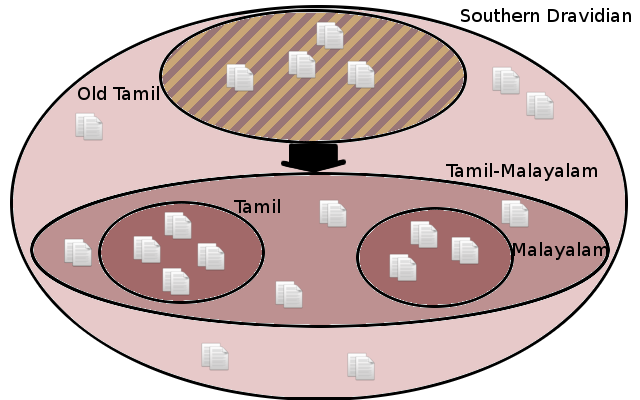
\includegraphics[height=.3\textheight]{dravidian.png}
\caption{The relation between Old Tamil and Tamil-Malayalam. Old Tamil is a historical variety whose breakup is the non-terminal languoid Tamil-Malayalam, which contains the terminal languoids Tamil and Malayalam. Lectodocs can be associated with any of these varieties, either directly or indirectly.}
\label{fig:dravidianbreakup}
\end{figure}

\subsubsection{The definition of Proto-Dravidian}
The above example has illustrated how to deal with a historical variety within a language family.  In some cases, we have to assume that the languoid under discussion is outside the language family. This is the case for proto-languages of a whole family, e.g. Proto-Dravidian. These are by definition not part of the family whose latest common ancestor they are. Table \ref{tab:protodravidiandocs} lists some lectodocs for Proto-Dravidian.

\begin{table}
\begin{tabular}{p{5cm}p{2cm}p{2cm}p{4cm}}
Lectodoc & Doculect & Terminal languoid & Non-terminal languoids\\ 
\hline
William Bright  (1986) Archaeology, linguistics, and ancient Dravidian
& Proto-Dravidian of Bright 1986 & Proto-Dravidian & - \\\\
Levi, Sylvain and Przyluski, Jean and Bloch, Jules  (1929) Pre-Aryan and pre-Dravidian in India
& Proto-Dravidian of Levi, Przyluski \&  Bloch 1929 & Proto-Dravidian & - \\\\
\end{tabular}
\caption{Some works which refer to the historical languoid `Proto-Dravidian'}
\label{tab:protodravidiandocs}
\end{table}

The breakup relation described above can also be applied to the relationship between Proto-Dravidian and Dravidian. Figure \ref{fig:protodravidian} illustrates this. 

\begin{figure}
 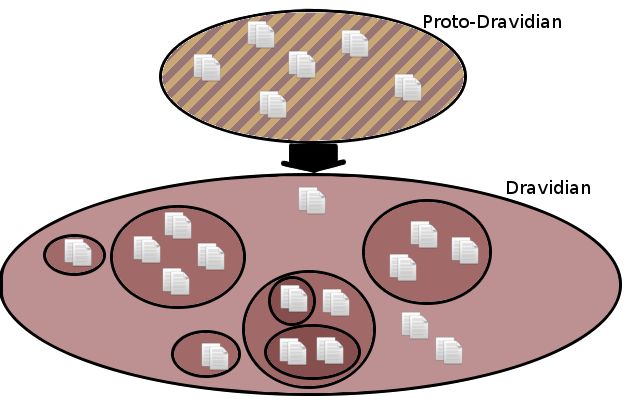
\includegraphics[height=.3\textheight]{protodravidian.png}
\caption{A top-level family as the result of the breakup of  a proto-language which his not a  member of a family itself. This case is illustrated by Proto-Dravidian.}
\label{fig:protodravidian}
\end{figure}

%         Annamalai describes Tamil
%         Annamalai descibes Old Tamil
%         Annamalai describes Dravidian
%         Annamalai describes Proto-Dravidian


\textbf{Theorems}\\
\ea All terminal languoids found in the breakup set of a historical variety are later varieties of the historical variety\z

\ea No nonterminal languoid found in the breakup set of a historical variety is  a later variety of the historical variety\z


\subsection{A note on dialects}
Note that not everything which is currently seen as a language automatically corresponds to a terminal languoid. This is most notable the case for the so-called macro-languages, like Arabic, Kurdish, or Quechua. These macro-languages are important at a social level, and speakers often identify with them, claiming to be a member of this linguistic group. At the same time, mutual intelligibility is often low, and the various varieties of Arabic for instance can be considered languages in their own right. This means that `Arabic' is not a terminal languoid, but a nonterminal languoid, as it subsumes a number of subvarieties. The relation between the Arabic dialects and the macro-language Arabic is thus the same (in a set-theoretic sense) as the relation between the macro-language Arabic and Semitic.

The same hold mutatis mutandis for dialects of English. There are abundant descriptions of English dialects, which can be grouped into non-terminal dialects. The languoid `English' then contains all those subsets, and is therefore nonterminal. Note that `English' is used here as a label for a set of varieties, and is distinct from `Standard English', which \em is \em a terminal languoid. This terminal languoid `Standard English' is itself a subset of the non-terminal languoid `English'.\footnote{In order to avoid confusion, one could choose `Angloid' as a label instead of `English' to highlight the set nature of the concept.}

\subsection{A note on historic dialects}
There are cases where we have a succession of historical varieties without necessarily a break-up stage in between. Archaic Latin and Classical Latin are for instance normally seen as continuations of the same language without intervening speciation. The model discussed here does not allow for such direct successions. Instead, it assumes a breakup of Archaic Latin into a very small family consisting only of Classical Latin, a singleton family so to speak. This has the advantage that the model does not have to be changed if a sister of Classical Latin were to be found. Hard-coding of the succession relationship between Archaic Latin and Classical Latin would require remodeling upon the discovery of such new knowledge, which is undesirable from an information science point of view.


\section{Types of languoids}

After this basic introduction, we can now engage in a more formal representation of the different types of languoids. Table \ref{tab:languoidhierarchy} shows the hierarchy of languoid types.

\begin{figure}
\Tree   [.languoid   [.terminal [.living \textbf{living\ language}\\(Kölsch) ] [.extinct [.without\ offspring \textbf{extinct\ lineage}\\(Gothic) ] [.with\ offspring \textbf{paleolect}\\(Latin,Proto-Dravidian) 
%  attested reconstructed 
] ] ] [.nonterminal \textbf{family}\\(Germanic) ]  ] 
\caption{Hierarchy of languoids with types and examples.}
\label{fig:languoidhierarchy}
\end{figure}

Basing ourselves on the criteria [$\pm$terminal], [$\pm$extinct],[$\pm$offspring], we can establish four types of languoid:
\textbf{Families} are non-terminal languoids. Terminal languoids are divided into \textbf{living languages}, which do have speakers, and historic varieties, which do not have speakers. Historic varieties are in turn divided into \textbf{extinct lineages} without any offspring and \textbf{paleolects}, which are the ancestor of at least one other terminal languoid.

These four types of languoids can be dinstinguished by a number of properties, which are listed in table \ref{tab:properties}.

\begin{table}
\begin{center}
  \begin{tabular}{lllll}
  & living & extinct lineage & paleolect & family\\
  \hline
  contains other languoids & -- & -- & -- & +\\
  has speakers & + & -- & -- & +/--\\
  has scatter & -- & -- & + & --\\
  \end{tabular}
\caption{Properties of languoids}
\label{tab:properties}
\end{center}
\end{table}

Only a family can contain other languoids, a logical corollary of the other languoids being terminal. The prime example of a languoid with speakers is the living language. A family can also have speakers if it contains at least one living language. If it contains only paleolects and extinct lineages as languoids, it does not have any speakers. The third and final concept is `scatter'. This refers to the breakup of a paleolect into a new language family. It is thus the 
projection of a terminal languoid on a non-terminal languoid, as discussed above for Old Tamil and Proto-Dravidian.

These three criteria provide operational definitions for the classifications of languoids into the four types.

These types themselves can enter in relations with each other as shown in table \ref{tab:languoidrelations}


\begin{table}
\begin{center}
\begin{tabular}{lllll}
  & living & extinct lineage & paleolect & family\\
living & / & / & succession & inclusion\\
extinct lineage & / & / & succession & inclusion\\
paleolect & / & / & succession & inclusion\\
family & / & / & scatter & inclusion
\end{tabular}
\caption{Relations between languoids. The `lower' varieties are on the left and the `higher' varieties are on top.}
\label{tab:languoidrelations}
\end{center}
\end{table}


We see that living languages and extinct lineages cannot be found on the `older' part of the relations. What is found on the `older' part are paleolects and families. Families can inlcude any of the other types of languoids. The relation between paleolects on the one hand and living languages or extinct lineages is one of succession. The relation between paleolects and families is called `scatter' here, i.e. the result of breakup. We thus have to model three relations: inclusion, scatter, and succession. Additionally, we have to get back to the doculect/lectodoc issue and find a formal modeling for this as well.

\section{Mathematical modeling}
In the following, we will use $L$ to denote a languoid, $p$ to denote a paleolect, $dl$ to denote a doculect and $ld$ to denote a lectodoc. Subscript $t$ and $nt$ refer to terminal and nonterminal languoids, respectively.

\subsection{Inclusion}
$L_{t} \subset L_{nt}$

$L_{nt} \subset L_{nt}$

\subsection{Scatter}
$p \prec L_{nt}$\prec

\subsection{Succession}
$p \prec L_{nt}; L_{t} \subset L_{nt} $

\subsection{Doculects}
$dl \in L $

\subsection{Lectodocs}
$ld \^= dl $
$ld \twoheadleftarrow  dl$ every lectodoc describes at least one doculect, potentially more
$dl \twoheadrightarrow ld$ every doculect is described by exactly one lectodoc

\section{Ontological modeling in the Semantic Web}



\subsection{Overview}
intro OWL
concepts 
instances

\subsection{inclusion}
skos:broader
skos:narrower

reflexive +
transitive (transitivebroader) +
symmetric -

\subsection{elementof}
rdf:a

reflexive -
transitive -
symmetric -

\subsection{precedence}
$\prec$
reflexive -
transitive -
symmetric -

\subsection{equivalence}
$ \^=   $

powder:describes


reflexive -
transitive -
symmetric -

\subsection{Succession}

$p \prec L_{nt}; L_{t} \subset L_{nt} $
reasoner

reflexive -
transitive +
symmetric -

\subsection{Other reasoners}
Latest common ancestor
Empirical grounding	

\section{Glottolog}
\section{conclusion and outlook}
    outlook
        extension to areal linguistics



\end{document}
